\documentclass[11pt,a4paper]{article}

% Packages for formatting and layout
\usepackage{geometry}  % Adjust margins
\geometry{margin=0.7in}
\usepackage{setspace}  % For line spacing
\usepackage{graphicx, wrapfig}
\graphicspath{ {./assets/} }
\usepackage{amsmath}   % For mathematical expressions
\usepackage{hyperref}  % For hyperlinks
\usepackage{enumitem}  % For custom lists

% Title information
\title{Predicting news truthfulness through graph-based retweet patterns.}
\author{Baggio Davide 2122547 \\ Martinez Zoren 2123873 \\ Brocheton Damien 2133034}
\date{}

\usepackage{etoolbox}
\makeatletter
\patchcmd{\@maketitle}{\null\vskip 2em}{}{}{}
\makeatother

\begin{document}

% Title Page
\maketitle

\section*{Motivation}

The rise of misinformation on social media has significant implications for public opinion, health, and safety, making it crucial to distinguish real news from fake. Twitter, as a major news source, often spreads information rapidly, sometimes without verification. By analyzing the graph structure of news propagation on Twitter, we can identify patterns in how real and fake news spread. This project aims to develop insights and tools to enhance the credibility of online information, contributing to a more informed and resilient public.
Recent studies\cite{rec_studies} have shown that machine learning models can effectively detect real or fake news by analyzing user-specific data, such as the profiles of those sharing the information. One of the biggest catches is the complexity of the generated models, mostly being Convolutional Neural Networks applied to Graphs and the low accuracy given new data. In this project, however, we aim to explore whether it’s possible to classify news as real or fake based solely on the "pure" retweet graph structure, independent of user metadata. By employing the algorithms outlined in the following sections, we will extract essential features from the retweet graph that can serve as inputs for a machine learning model, enabling an analysis based purely on the patterns of information spread.

\subsection*{Dataset}

The dataset is part of a bigger pool provided by the Twitter API. This part is shared on github under the Apache Licence, Version 2.0\cite{dataset}. The dataset is well documented in this paper\cite{data_paper}. It is basically a Graph with many connected components, each representing a news tree, composed of the main tweet of the news and all the retweets associated with it.

\section*{Method}

\subsection*{Problem}
Our objective is to identify the characteristics of tweets that reference a fake news, and determine if a new tweet references it by looking at its characteristics.
To analyze the dataset, we need to construct the graph from the dataset. The structure is represented as follows:
\newline
\begin{wrapfigure}{r}{0.5\textwidth}
	\begin{center}
	  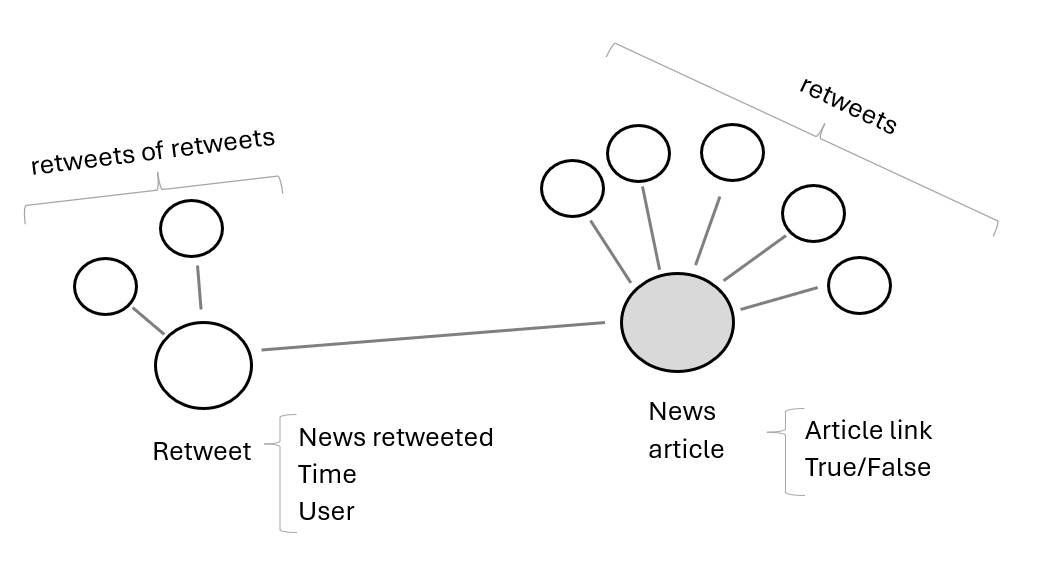
\includegraphics[width=0.48\textwidth]{struct}
	\end{center}
\end{wrapfigure}
\begin{itemize}
	\setlength\itemsep{-0.3em}
	\item \textbf{Graph Type}: Tree-structured graphs
	\item \textbf{Root Node}: News item (labeled true/false)
	\item \textbf{Other Nodes}: Twitter users who retweeted the news
	\item \textbf{Edges}:
	\begin{itemize}
		\setlength\itemsep{-0.3em}
		\item News item $\leftrightarrow$ User: Direct retweet
		\item User $\leftrightarrow$ User: Retweet through an intermediary
	\end{itemize}
	\item \textbf{Additional Information}: Retweet timestamps
\end{itemize}

The goal is to extract features from the network and use that data to train a machine learning model to predict the truthfulness of news.
The algorithms that we are going to use are important for:
\begin{itemize}
	\setlength\itemsep{-0.3em}
	\item \textbf{Average depth of trees}: Is the depth of the trees greater for fake news?
	\item \textbf{Average retweet breadth}: Do fake news tend to spread more quickly having a greater breadth at the first level?
	\item \textbf{Average time between retweets}: Do fake news spread faster?
	\item \textbf{Peak diffusion time}: Do fake news have an explosive peak?
	\item \textbf{Users reliability score}: various features based on the ranking of users who shared the news
	\item \textbf{Centrality and Pagerank}: What nodes are more common to find in paths between other 2 nodes?
\end{itemize}

\section*{Intended Experiments}

\subsection*{User reliability ranking}
\begin{wrapfigure}{r}{0.5\textwidth}
	\begin{center}
	  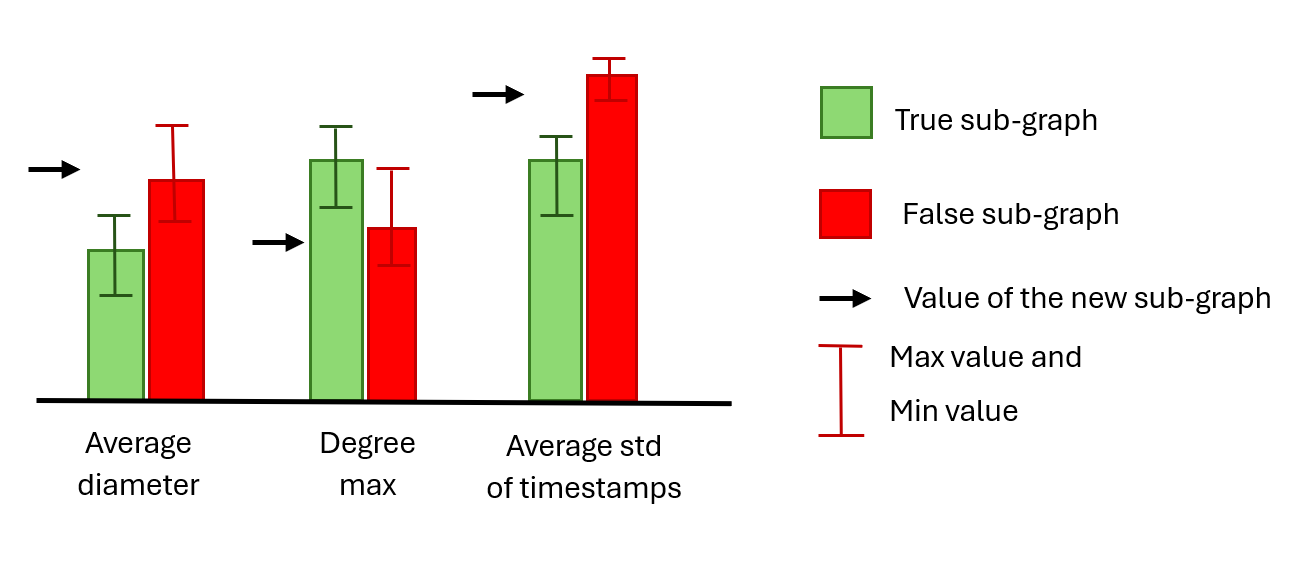
\includegraphics[width=0.48\textwidth]{results}
	\end{center}
\end{wrapfigure}
One of the goal is to visualize wether new data involving a news fits better into the "Real news" or "Fake news" category. This can be achieve displaying a bar graph representing the features studied previously.\\
The final step is to create a ranking of users based on their reliability and to generate features for the data using this ranking. To do this, the following factors will be considered:
\begin{itemize}
	\setlength\itemsep{-0.3em}
	\item Number of retweets of false news
	\item Percentage of retweets of true vs. false news
	\item Betweenness centrality of the user in the graph
	\item Pagerank of the user in the graph
\end{itemize}

For large datasets computing the ranking for ALL users might be computationally expensive. Therefore, in this case, users with good centrality measures will have priority. 
The features of the news obtained from this ranking are as follows:
\begin{itemize}
	\setlength\itemsep{-0.3em}
	\item Average Ranking Positions of users who retweeted the news
	\item Percentage of reliable users (e.g. percentage of users in the top 20)
	\item Minimum and maximum position
	\item Weighted score based on reliability
\end{itemize}

\subsection*{Machine learning models}

The models we want to try are the following:
\begin{itemize}
	\setlength\itemsep{-0.3em}
	\item \textbf{Support Vector Machine}
	\item \textbf{Feed Forward Neural Network}
	\item \textbf{Random Forest}
\end{itemize}

We will make comparisons to better understand which model fits this problem best, based on which one achieves better accuracy and also the time it will take to train it.
\\\textbf{Libraries}: Networkx\cite{networkx} (for Graph analysis), Scikit-Learn (for SVM and RF models), Pytorch (for FFNN model)
\\\textbf{Evaluation metrics of the model}: Accuracy, Precision, Recall and F1-Score
\\\textbf{Machine for experiments}: 
\begin{itemize}
	\setlength\itemsep{-0.3em}
	\item AMD Ryzen 5 3500U (8-cores), 8GB DDR4, Windows 11 or Ubunutu 20.04
	\item AMD Ryzen 5 4500 (8-cores), Radeon RX 6600, 16GB DDR4, Windows 11 or Ubuntu 20.04
\end{itemize}

\newpage

\begin{thebibliography}{9}
	\bibitem{rec_studies} Yi Han, Shanika Karunasekeran, Christopher Leckie\\"Graph Neural Networks with Continual Learning for Fake News Detection from Social Media",\\ \url{https://arxiv.org/pdf/2007.03316}, 2020.
	\bibitem{dataset} Dataset: \url{https://github.com/safe-graph/GNN-FakeNews/tree/main},\\\url{https://drive.google.com/drive/folders/1OslTX91kLEYIi2WBnwuFtXsVz5SS_XeR?usp=sharing}
	\bibitem{data_paper} Kai Shu, Deepak Mahudeswaran, Suhang Wang, Dongwon Lee and Huan Liu\\"FakeNewsNet: A Data Repository with News Content, Social Context and Spatiotemporal Information for Studying Fake News on Social Media",\\ \url{https://arxiv.org/pdf/1809.01286}, 2019
	\bibitem{networkx} NetworkX library: \url{https://networkx.org/documentation/stable/}
\end{thebibliography}

\newpage

\section*{Contribution}
Contributors:
\begin{itemize}
	\setlength\itemsep{-0.3em}
	\item Baggio Davide ($\frac{1}{3}$ of the work): Finding a well documented dataset, reading the related papers and understanding it. Writing the first part of the proposal and preprocessing the dataset ready for analysis into a python script.
	\item Martinez Zoren ($\frac{1}{3}$ of the work): Finding a well documented dataset,  reading the related papers and understanding it. Writing the third part of the proposal and planning on the machine learning models to use in order to achieve the goal of the project.
	\item Brocheton Damien ($\frac{1}{3}$ of the work): Finding a well documented dataset,  reading the related papers and understanding it. Writing the second part of the proposal and starting to write the postprocessing of the data into a python script that compare new data with the studied one using a probabilistic algorithm.
\end{itemize}

\end{document}
